% Created 2024-10-27 Sun 18:58
% Intended LaTeX compiler: pdflatex
\documentclass[11pt]{article}
\usepackage[utf8]{inputenc}
\usepackage[T1]{fontenc}
\usepackage{graphicx}
\usepackage{longtable}
\usepackage{wrapfig}
\usepackage{rotating}
\usepackage[normalem]{ulem}
\usepackage{amsmath}
\usepackage{amssymb}
\usepackage{capt-of}
\usepackage{hyperref}
\author{Bryce MacInnis}
\date{\today}
\title{Visualizing Behavioural Traits of Quality-Diversity Algorithms with Natural Language Queries}
\hypersetup{
 pdfauthor={Bryce MacInnis},
 pdftitle={Visualizing Behavioural Traits of Quality-Diversity Algorithms with Natural Language Queries},
 pdfkeywords={},
 pdfsubject={},
 pdfcreator={Emacs 29.3 (Org mode 9.6.15)}, 
 pdflang={English}}
\begin{document}

\maketitle
\section{Background}
\label{sec:org13e1f2e}

In Reinforcement Learning, we're often interested in the best performing solution of a task domain. But understanding the entire fitness landscape of different strategies
is equally informative. Quality-diversity algorithms are a reinforcement learning methodology which aim
to solve a task domain with a population of diverse solutions instead of a single best-performing solution.

In this paper, we look at one particular instance of a Quality-Diversity algorithm, CMA-ME.
Which combines two earlier predecessor works, CMA-ES, a famous blackbox optimization algorithm
and the other MAP-Elites, which archives individuals in a population by their behavioural characteristics.
In this combination, CMA-ME, uses CMA-ES to optimize a neural network to find competitive policies (methods
of interacting with the environment) to optimize the reward achieved and CMA-ME uses MAP-Elites to archive
the best performing solutions by their behavioural characteristics, such that a diverse set of strategies
are 

\section{Problem Statement}
\label{sec:orge903137}

In this paper, we make a novel contribution of combining the fitness landscape found by the CMA-ME algorithm
and we bolt on natural language processing capabilities in order to analyze the strategies found.
This contribution serves two purposes. First, since the behavioural space is often complex and high-dimensional,
adding the ability to query the space with natural language improves the researcher's ability to make sense of the
strategies. Secondly, by integratnig natural language processing, we expand the edge of what is possible and provide
an entry point to other researches interested in the intersection of natural language processing and reinforcement learning
reducing the barrier to entry and hopefully generating some interest in the process.

\begin{figure}[htbp]
\centering
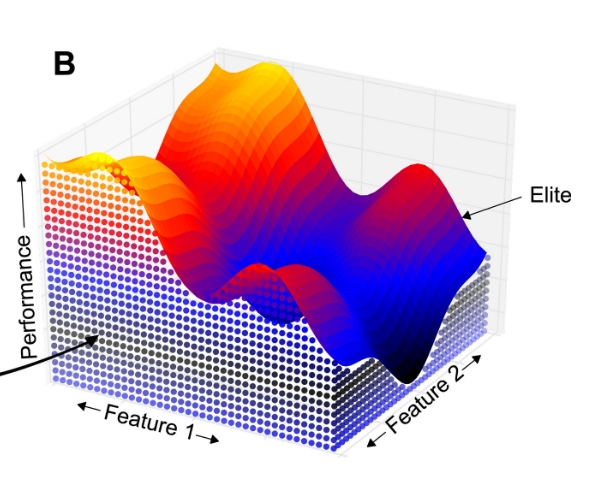
\includegraphics[width=.9\linewidth]{./map-elites.png}
\caption{The behavioural space captured by MAP-Elites}
\end{figure}

\begin{figure}[htbp]
\centering
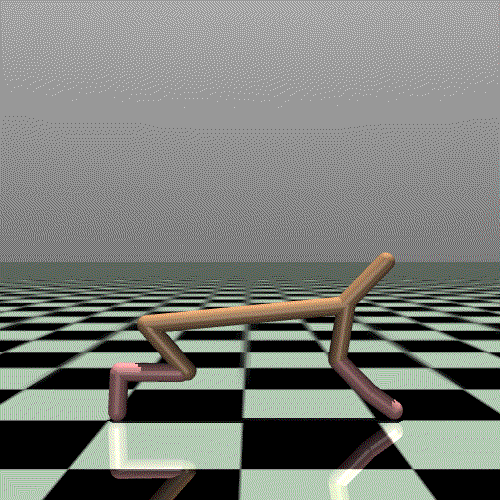
\includegraphics[width=100px]{./half_cheetah2.png}
\caption{Mujoco's HalfCheetah environment}
\end{figure}

\begin{figure}[htbp]
\centering
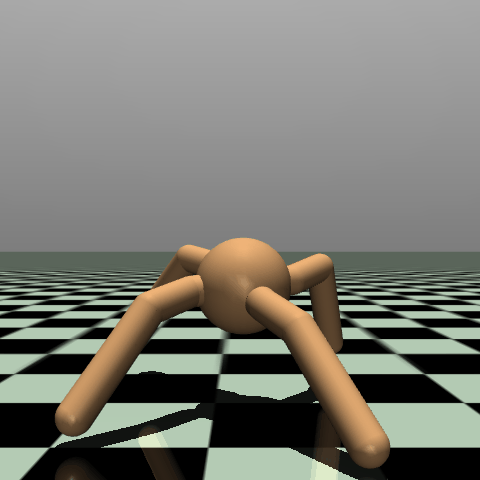
\includegraphics[width=100px]{./ant2.png}
\caption{Mujoco's Ant environment}
\end{figure}

\section{Related Work}
\label{sec:org11c1eed}

In Salimans et al., Evolution Strategies are applied as an alternative paradigm to neural networks
in reinforcement learning. They found that evolutionary algorithms are competitive with state-of-the-art
gradient-based methods and invigorated research in the direction of evolutionary algorithms. 

In Colas et. al, (Colas, Cédric and Madhavan, Vashisht and Huizinga, Joost and Clune, Jeff, 2020) they apply the MAP-Elites algorithm against the Mujoco's Ant environment. In their work,
they characterize the behavioural axes of the MAP-Elites by the proportion of the time that each leg comes into
contact with the ground. They also investigate the role of quality-diversity algorithms for damage recovery in robotics tasks.
They do so by altering the Mujoco simulator to prevent the control of joints. In this case, they investigate
if it is possible for the robotic controller to switch from a balanced 4-legged policy to a 3-legged policy
without the damaged leg.

In Tjanaka et al, they provide \emph{pyribs} (Tjanaka, Bryon and Fontaine, Matthew C and Lee, David H and Zhang, Yulun and Balam, Nivedit Reddy and Dennler, Nathaniel and Garlanka, Sujay S and Klapsis, Nikitas Dimitri and Nikolaidis, Stefanos, 2023), an implementation of the CMA-ME algorithm that combines the CMA-ES blackbox optimization method with
the MAP-Elites archive. In this paper, \emph{pyribs} is used to collect the training dataset for the HalfCheetah and Ant environments.

\section{Methodology}
\label{sec:org64b4ed7}

The following goals for this project are identified, and will be completed in this order as much as possible
before the deadline.

\begin{enumerate}
\item Self-labelling individuals: Given a point in the behavioural space, generate a natural language description
of the individual's capabilities.

\item Natural language queries: Given a natural language description/query, return the nearest individual
matching the description.

\item Regional queries: Given a natural language description, as before, return a subset of individuals
that match the description.

\item Visualization: Given a query that selects a region of the behavioural space, illuminate the behavioural
space graph with the search region.
\end{enumerate}

\section{Project Plan}
\label{sec:org5f53c15}

Week of October 28th

The training data will be collected using the \emph{pyribs} implementation of CMA-ME.
The first batch of data will include 
Then a dataset of labels/templates will be created using a large language model (GPT).

Week of November 4th

During this week, model training will begin in training the self-labelling implementation.
Then the converse


Week of November 11th

Reading Week (I'm going on vacation)

Week of November 18th



Week of November 25th

Time reserved for collecting figures and writing the presentation and final report.

\section{References}
\label{sec:org0b9e514}

\noindent
Colas, Cédric and Madhavan, Vashisht and Huizinga, Joost and Clune, Jeff (2020). \emph{Scaling MAP-Elites to deep neuroevolution}, ACM.

\noindent
Tjanaka, Bryon and Fontaine, Matthew C and Lee, David H and Zhang, Yulun and Balam, Nivedit Reddy and Dennler, Nathaniel and Garlanka, Sujay S and Klapsis, Nikitas Dimitri and Nikolaidis, Stefanos (2023). \emph{Pyribs: A Bare-Bones Python Library for Quality Diversity Optimization}, Association for Computing Machinery.
\end{document}
